\chapter{Présentation de l'organisme d'accueil et contexte du projet}
\label{cp:introduction}

\textit{Avant de conduire un projet au sein d'une entreprise, il est indispensable d'en appréhender l'organisation et les champs de compétence. Ce chapitre présente le groupe Segula Technologies, avec un focus particulier sur sa filiale marocaine, cadre principal du stage. Il se conclut par une présentation de la méthodologie DMAIC retenue pour structurer l'ensemble de la démarche projet.}

%%%%%%%%%%%%%%%%%%%%%%%%%%%%%%%%%%%%%%%%%%%%%%%%%%%%%%%%%%%
%%  SECTION I — SEGULA TECHNOLOGIES
%%%%%%%%%%%%%%%%%%%%%%%%%%%%%%%%%%%%%%%%%%%%%%%%%%%%%%%%%%%
\section{Segula Technologies}

%% ---- I.1 Présentation ----
\subsection{Présentation de Segula Technologies}

Segula Technologies est un groupe d'ingénierie international spécialisé dans l'innovation et le développement industriel. Créée en 1985, l'entreprise accompagne les grands acteurs industriels dans divers secteurs tels que l'aéronautique, l'automobile, l'énergie, le ferroviaire, le naval et la santé. L'entreprise se distingue par son engagement envers l'innovation, avec plus de 130 projets de R\&D chaque année, couvrant des domaines comme l'intelligence artificielle, la fabrication additive et la transition énergétique.

\begin{figure}[H]
    \centering
    
\includegraphics[width=0.5\linewidth]{segula-logo.png}
    \caption{Logo de la société}
    \label{fig:segula-logo}
\end{figure}

Comme illustré dans la \autoref{fig:segula-logo}, Segula Technologies est présent dans 30 pays, fort de ses 140 implantations dans le monde, le groupe privilégie une relation de proximité avec ses clients grâce aux compétences de ses 15 000 collaborateurs afin de concevoir des solutions technologiques avancées et améliorer la compétitivité de ses clients en menant des projets d'envergure, allant des études jusqu'à l'industrialisation et la production.

\begin{figure}[H]
    \centering
    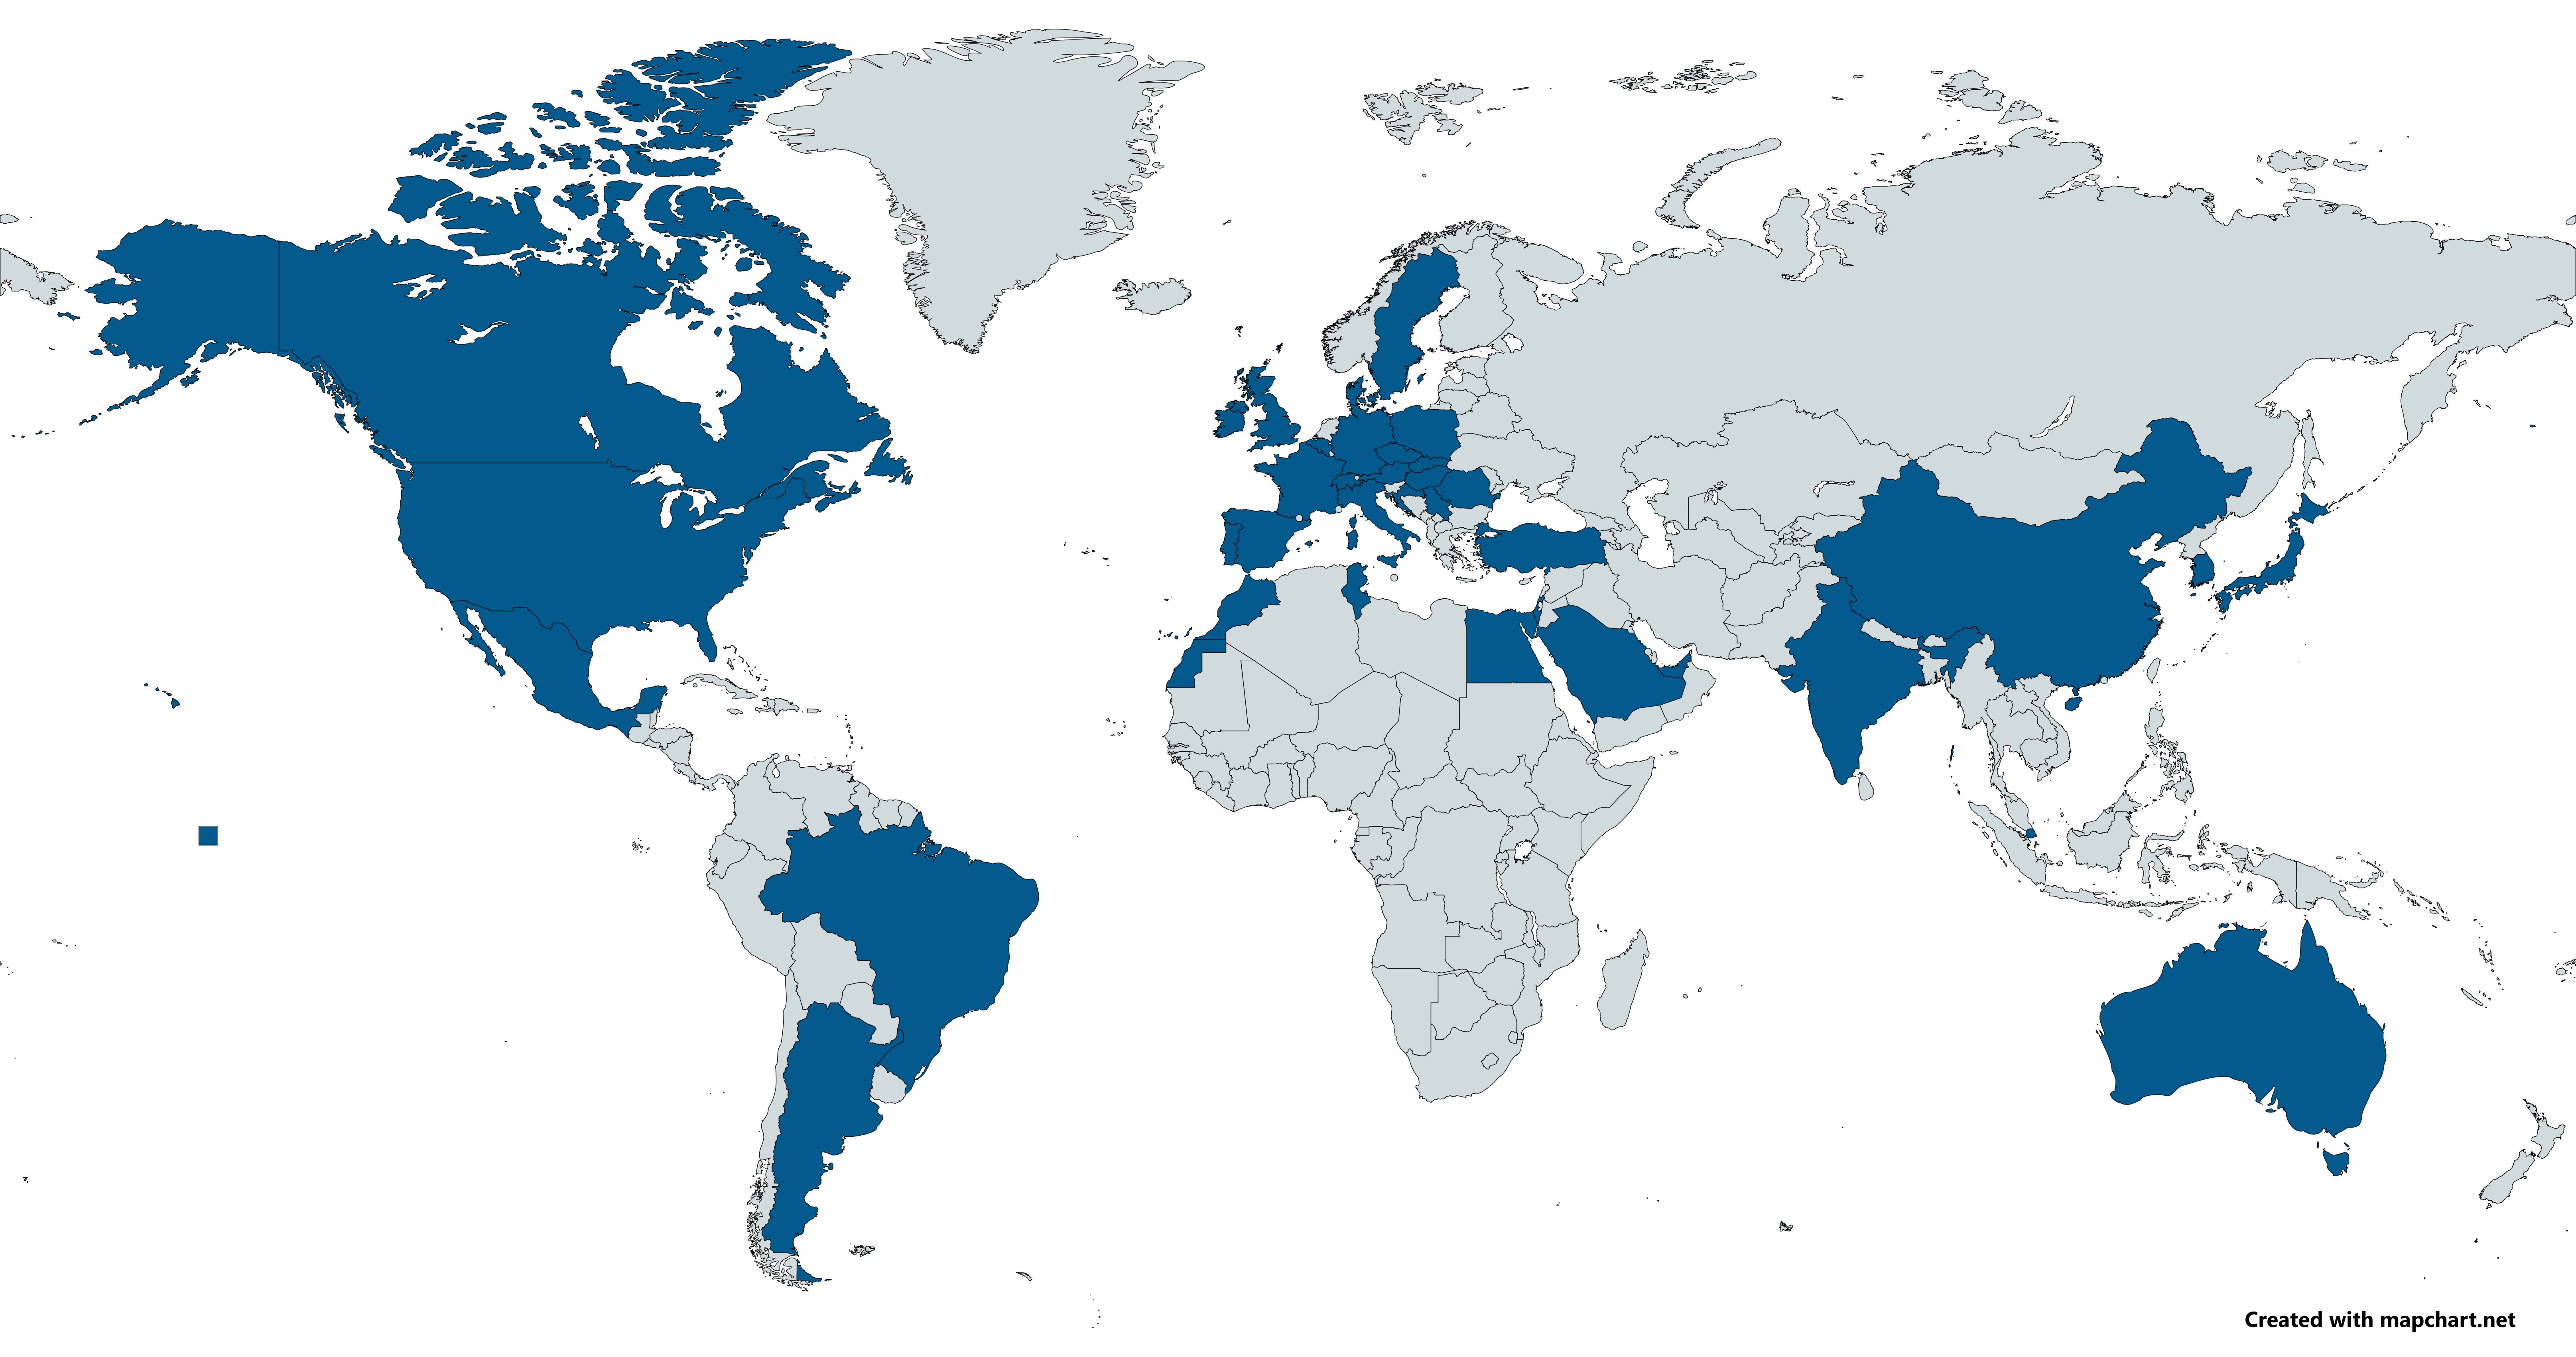
\includegraphics[width=0.9\linewidth]{Figures/introduction/map.png}
    \caption{Implantation du Groupe Segula Technologies dans le monde}
    \label{fig:segula-worldwide}
\end{figure}

La \autoref{fig:segula-worldwide} illustre la présence mondiale de Segula Technologies avec ses implantations dans les régions suivantes:

\begin{table}[H]
    \caption{Implantations de Segula Technologies par région}
    \label{tab:implantations-regions}
    \centering
    \begin{tabularx}{\textwidth}{|>{\bfseries\centering\arraybackslash}p{3.5cm}|X|}
        \hline
        \mdseries{Région} & \centering\mdseries{Pays} \tabularnewline
        \hline
        Amériques & Argentine, Brésil, Canada, États-Unis, Mexique \\
        \hline
        Asie-Océanie & Australie, Chine, Corée du Sud, Inde, Japon, Singapour \\
        \hline
        Afrique – Moyen Orient & Arabie Saoudite, Égypte, Émirats arabes unis, Israël, Maroc, Tunisie, Turquie \\
        \hline
        Europe & Allemagne, Autriche, Belgique, Croatie, Danemark, Espagne, France, Hongrie, Irlande, Italie, Pologne, Portugal, République tchèque, Roumanie, Royaume-Uni, Serbie, Slovaquie, Suède, Suisse \\
        \hline
    \end{tabularx}
\end{table}

\subsubsection*{Segula Technologies Maroc}

SEGULA Technologies Maroc est une filiale du groupe SEGULA Technologies en Afrique, créée en 2007. Grâce à ses bureaux d'études à Casablanca et à Agadir, ainsi sa filiale SIMRA. La filiale marocaine emploie plus de 700 ingénieurs et techniciens hautement qualifiés, avec un fort chiffre d'affaires plus de 22 millions d'euros en 2021. La filiale a travaillé sur la conception et l'industrialisation de nouveaux produits ou nouvelles usines pour ses clients. Elle offre des services d'ingénierie et de conseil pour la conception de véhicules, l'optimisation des processus de production, la gestion de la chaîne d'approvisionnement, l'analyse des coûts, la simulation et la modélisation.

\begin{figure}[H]
    \centering
    
\includegraphics[width=0.4\textwidth]{Figures/SIMRA.png}
    \caption{Logo de SIMRA - filiale de Segula Technologies Maroc}
    \label{fig:simra-logo}
\end{figure}

%% ---- I.2 Fiche technique ----
\subsection{Fiche technique}

Le \autoref{tab:fiche-technique} présente en détails l'ensemble des informations sur l'entreprise d'accueil :

\begin{table}[H]
    \caption{Fiche technique de Segula Technologies}
    \label{tab:fiche-technique}
    \centering
    \begin{tabularx}{\textwidth}{|>{\bfseries\raggedright}p{4.5cm}|X|}
        \hline
        \mdseries{Raison sociale} & SEGULA Technologies \\
        \hline
        \mdseries{Forme juridique} & Société par actions simplifiée \\
        \hline
        \mdseries{Année de création} & 1984 \\
        \hline
        \mdseries{Adresse postale} & 19 Rue d'Arras 92000 Nanterre, France \\
        \hline
        \mdseries{Activité} & Ingénierie, études techniques \\
        \hline
        \mdseries{Chiffre d'affaires (2023)} & 27 142 440 € \\
        \hline
        \mdseries{Implantations} & +140 implantations \\
        \hline
        \mdseries{Site web} & www.segulatechnologies.com/fr \\
        \hline
    \end{tabularx}
\end{table}

%% ---- I.3 Activités ----
\subsection{Activités}

Segula Technologies est le premier groupe européen de conseil et d'ingénierie en innovation technologique. Le groupe couvre toutes les phases du cycle de vie d'un projet, de sa définition (veille technologique, études de faisabilité technique, définition des stratégies, etc.) à sa concrétisation (conception, mise en œuvre et validation de solutions, etc.). L'activité s'organise autour de 2 axes :

\begin{itemize}
    \item[•] Conseil en technologie et en recherche \& développement.
    \item[•] Conseil en organisation et en systèmes d'information.
\end{itemize}

%% ---- I.4 Domaines d'intervention ----
\subsection{Domaines d'intervention}

Le groupe Segula Technologies travaille sur différents secteurs dont le secteur industriel et le secteur tertiaire. Au sein du secteur industriel, il joue un rôle très important en étant porté sur plusieurs domaines : l'automobile, l'aéronautique, le naval, le ferroviaire, l'énergie, et encore le pharmaceutique.

\begin{figure}[H]
    \centering
    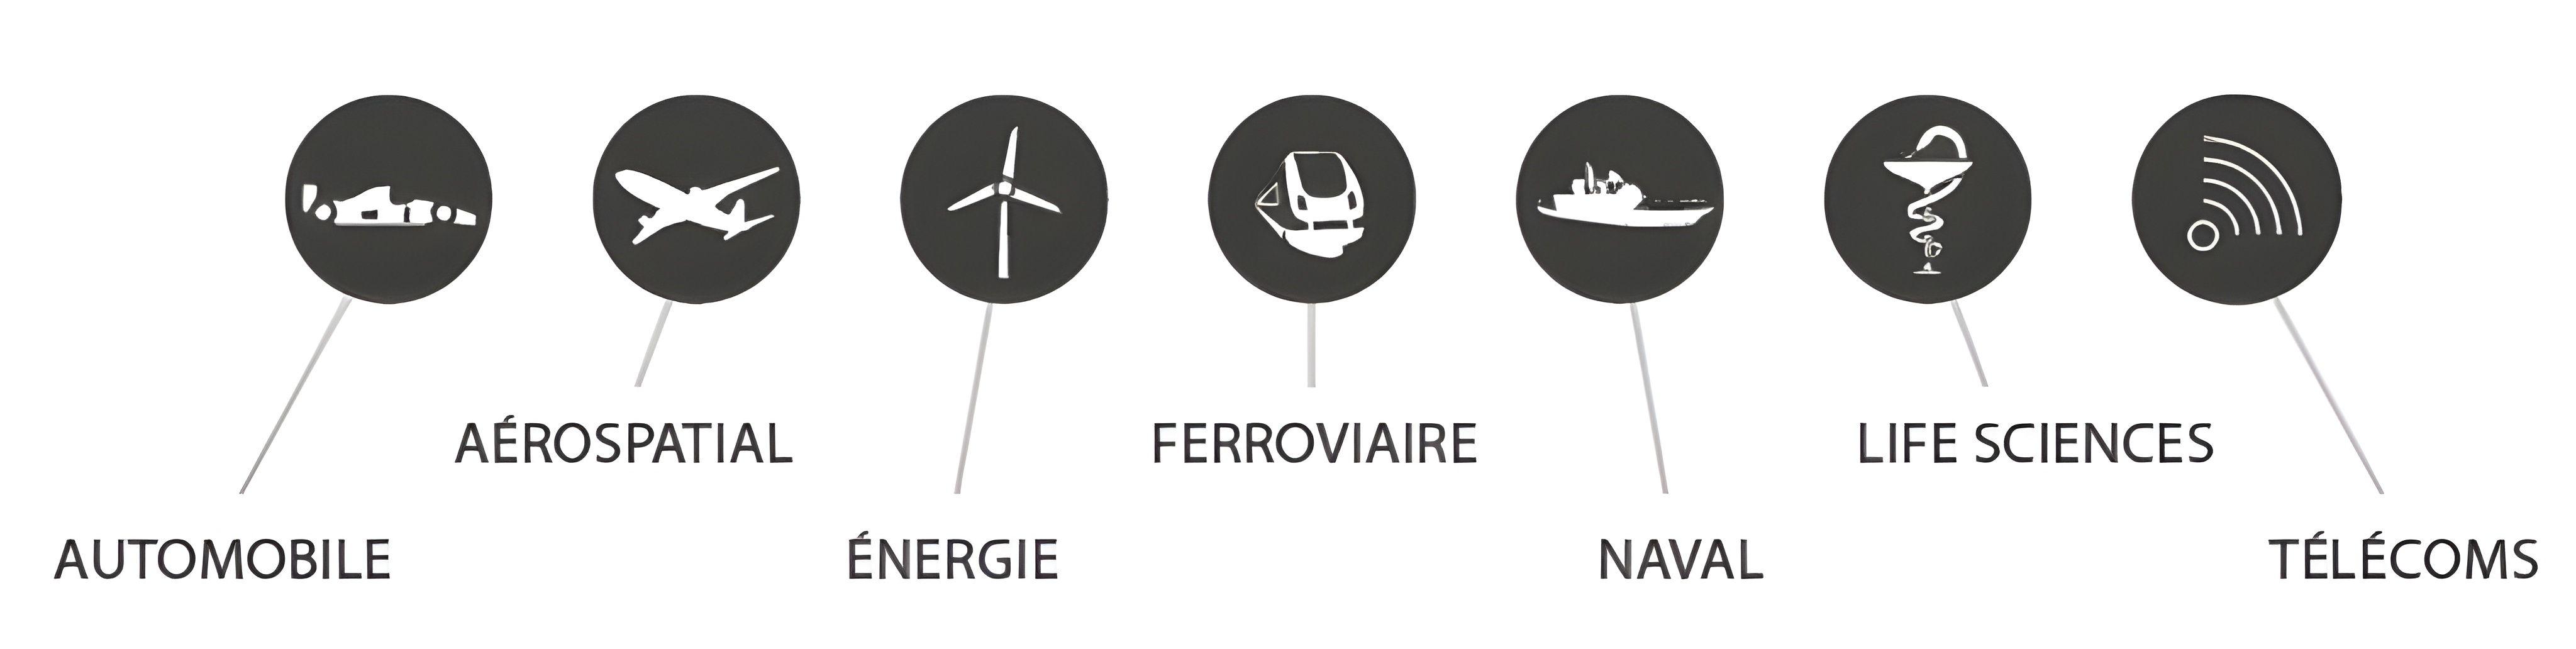
\includegraphics[width=0.9\linewidth]{Figures/introduction/domaines.png}
    \caption{Les divers secteurs d'activité de SEGULA Technologies}
\end{figure}

%% ---- I.5 Clients ----
\subsection{Clients}

Segula Technologies travaille avec une diversité de clients dans plusieurs secteurs, notamment l'automobile, l'aéronautique et le ferroviaire. En aéronautique, elle collabore avec des leaders de l'industrie pour développer des technologies avancées et optimiser la production. Dans le ferroviaire, Segula soutient des entreprises majeures en offrant des solutions innovantes pour le transport sur rail.

Dans le secteur automobile, l'un des principaux clients de Segula Technologies est Stellantis né de la fusion entre PSA (Peugeot Société Anonyme) et FCA (Fiat Chrysler Automobiles), qui englobe les marques Peugeot, Citroën, DS, Opel et Vauxhall. En 2014, PSA détenait une part de marché de 11,8 \% en Europe, démontrant son influence et son importance dans l'industrie automobile.

Le \autoref{tab:clients-partenaires} présente les principaux clients et partenaires de Segula Technologies classés par secteur d'activité.

\begin{table}[H]
    \caption{Principaux clients et partenaires de Segula Technologies}
    \label{tab:clients-partenaires}
    \centering
    \renewcommand{\arraystretch}{1.8}
    \begin{tabularx}{\textwidth}{|>{\centering\arraybackslash}p{2.8cm}|X|}
        \hline
        \mdseries{Secteur} & \centering\mdseries{Clients / Partenaires} \tabularnewline
        \hline
        & \centering
          
\includegraphics[height=0.5cm]{Figures/logos-partners/cars/Stellantis.png} \hspace{0.3cm}
          
\includegraphics[height=0.5cm]{Figures/logos-partners/cars/Peugeot.png} \hspace{0.3cm}
          
\includegraphics[height=0.5cm]{Figures/logos-partners/cars/Renault.png} \hspace{0.3cm}
          
\includegraphics[height=0.5cm]{Figures/logos-partners/cars/FIAT.png} \tabularnewline
        \mdseries{Automobile}
        & \centering
          
\includegraphics[height=0.5cm]{Figures/logos-partners/cars/DS.png} \hspace{0.3cm}
          
\includegraphics[height=0.5cm]{Figures/logos-partners/cars/opel.png} \hspace{0.3cm}
          
\includegraphics[height=0.5cm]{Figures/logos-partners/cars/Dacia.png} \hspace{0.3cm}
          
\includegraphics[height=0.5cm]{Figures/logos-partners/cars/Continental.png} \tabularnewline
        & \centering
          
\includegraphics[height=0.5cm]{Figures/logos-partners/cars/gestamp.png} \hspace{0.3cm}
          
\includegraphics[height=0.5cm]{Figures/logos-partners/cars/Plastic_Omnium.png} \hspace{0.3cm}
          
\includegraphics[height=0.5cm]{Figures/logos-partners/cars/avtovaz.jpg} \hspace{0.3cm}
          
\includegraphics[height=0.5cm]{Figures/logos-partners/cars/smrc.jpg} \tabularnewline
        \hline
        \mdseries{Aéronautique}
        & \centering
          
\includegraphics[height=0.5cm]{Figures/logos-partners/aero/Airbus.png} \hspace{0.3cm}
          
\includegraphics[height=0.5cm]{Figures/logos-partners/aero/Safran.png} \hspace{0.3cm}
          
\includegraphics[height=0.5cm]{Figures/logos-partners/aero/Stelia.png} \tabularnewline
        \hline
        \mdseries{Ferroviaire}
        & \centering
          
\includegraphics[height=0.5cm]{Figures/logos-partners/ferroviaire/Alstom.png} \hspace{0.3cm}
          
\includegraphics[height=0.5cm]{Figures/logos-partners/ferroviaire/Intelligent Energy.png} \tabularnewline
        \hline
    \end{tabularx}
\end{table}

%%%%%%%%%%%%%%%%%%%%%%%%%%%%%%%%%%%%%%%%%%%%%%%%%%%%%%%%%%%
%%  SECTION II -- METHODOLOGIE DE TRAVAIL
%%%%%%%%%%%%%%%%%%%%%%%%%%%%%%%%%%%%%%%%%%%%%%%%%%%%%%%%%%%
\section{Méthodologie de travail}

\subsubsection{Choix de la démarche appropriée}

Pour garantir le succès de ce projet, il est essentiel de sélectionner une méthodologie de travail adaptée permettant de gérer et de structurer les différentes étapes, depuis la définition du problème jusqu'à son analyse, puis la mise en œuvre de solutions. Parmi les approches couramment utilisées pour la résolution de problèmes dans l'industrie figurent le DMAIC, le PDCA et la méthode 8D. Ces méthodes peuvent être catégorisées selon deux critères principaux :

\begin{itemize}
    \item La taille du problème à résoudre (petite, moyenne ou grande).
    \item La nature de la stratégie adoptée : s'il s'agit d'un processus d'amélioration continue ou de la résolution d'un problème spécifique.
\end{itemize}

À l'issue de cette analyse comparative, nous constatons que la démarche DMAIC est la plus adaptée à notre situation, compte tenu de la complexité du problème traité et de notre objectif d'amélioration à long terme.

\subsubsection{Définition de la démarche DMAIC}

DMAIC fait référence à un cycle visant à améliorer, optimiser et développer la conception au sein d'un service. Cette démarche est basée sur une approche structurée en cinq étapes ordonnancées selon une logique rigoureuse. Chaque lettre composant l'acronyme DMAIC correspond à l'initiale de la fonction de l'étape correspondante :

\begin{itemize}
    \item \mdseries{Define (Définir)} : consiste à définir clairement les objectifs du projet, les besoins des clients, les exigences et les contraintes.
    \item \mdseries{Measure (Mesurer)} : consiste à rassembler les informations nécessaires pour traiter le sujet de façon objective, ainsi qu'à identifier les zones critiques.
    \item \mdseries{Analyze (Analyser)} : vise à analyser les données collectées pour identifier les causes racines des problèmes et les opportunités d'amélioration.
    \item \mdseries{Improve (Améliorer/Innover)} : porte sur le développement et la mise en œuvre de solutions dont les performances correspondent aux objectifs fixés.
    \item \mdseries{Control (Contrôler/Vérifier)} : consiste à vérifier la performance et à suivre les résultats des solutions mises en œuvre afin de pérenniser les gains obtenus.
\end{itemize}

\subsubsection{Outils utilisés}

Pour mener à bien ce projet, plusieurs outils logiciels ont été mobilisés, chacun répondant à un besoin spécifique du cycle de développement.

\paragraph{Conception et développement.}

\begin{figure}[H]
\centering
\begin{minipage}[t]{0.45\textwidth}
    \centering
    
\includegraphics[height=1.8cm]{Figures/tools/catia.png}\\[0.6em]
    \mdseries{CATIA V5}\\
    \textit{Modélisation 3D des pièces\\et exécution des macros}
\end{minipage}
\hfill
\begin{minipage}[t]{0.45\textwidth}
    \centering
    
\includegraphics[height=1.8cm]{Figures/tools/vs.png}\\[0.6em]
    \mdseries{Visual Studio}\\
    \textit{Développement et débogage\\des macros VBA / CATScript}
\end{minipage}
\end{figure}

\paragraph{Analyse des données.}

\begin{figure}[H]
\centering
\begin{minipage}[t]{0.45\textwidth}
    \centering
    
\includegraphics[height=1.8cm]{Figures/tools/excel.png}\\[0.6em]
    \mdseries{Microsoft Excel}\\
    \textit{Manipulation des données\\et rapports de conformité}
\end{minipage}
\hfill
\begin{minipage}[t]{0.45\textwidth}
    \centering
    
\includegraphics[height=1.8cm]{Figures/tools/latex.png}\\[0.6em]
    \mdseries{\LaTeX}\\
    \textit{Rédaction structurée du rapport\\avec gestion automatique des références}
\end{minipage}
\end{figure}
